\chapter{Datasets \& Transcribing}\label{ch:datasets}
\section{Datasets}
We use learning-based classification algorithms.
This means, given a set of rules, they try to induce the underlying patterns of a training set.
The resulting patterns are then used to classify unseen entities of a test set.
To train and test our algorithms we use two datasets, each consisting of labeled text pairs.
A pair has the label $True$ if both texts were authored by the same person and $False$ if not.\\\\
% PAN20 fan-fiction
First, we will use the small official dataset from the PAN2020 task on Authorship Verification from \cite{bevendorff2020overview}.
This allows us to compare our results to the other methods submitted.
It consists of 52.601 text pairs collected from the fanfiction website \url{fanfiction.net}.
The dataset file is formatted in the PAN20 format with each line containing a json object with the text pair, an ID, and optionally some additional information such as the corresponding fandoms\footnote{The franchise a fanfiction text belongs to. It can be seen as the topical domain of the text.}.
In contrast, the large official dataset contains 256.000 samples.
This is roughly five (4.86) times as many samples as the small data set.
Efforts have been made to maximally optimize the methods used, but due to some implementation details, the utilization of this dataset is infeasible for now.\\
% Gutenberg
We source the second dataset from \cite{stein2019unbiasedGutenbergCorpus}.
It presents a dataset containing science fiction and adventure texts from the 19th and 20th century, compiled from books from Project Gutenberg\footnote{\url{https://www.gutenberg.org/}}.
As discussed earlier, the aim of this dataset is to reduce common biases in data sets for Authorship Verification.
This makes it a good candidate for evaluating new authorship verifiers.
With only 262 text pairs, it is much smaller than the first dataset used.
% It is well suited for the much slower Unmasking algorithm, but might lead to overfitting.
To mitigate overfitting, we use out-of-fold cross-validation to evaluate the models instead of a standard train-test-split method.
This dataset is in the old PAN format\footnote{\textcolor{violet}{TBD: Used from PANXX to PANXX}} and is converted to the new PAN20 format for standardization\footnote{The code for the conversion is available at \url{https://github.com/torond/NAACL-19}}.\\

% Cleaning
% Describe FF cleaning
% g2p_en uses context -> Transcribe entire texts
% Phonetic algos transcribe word-wise -> Word separated

% Transcribing
% Repeat that the transcriptions are used as inputs
\section{Transcribing}
We use a range of open-source libraries to transcribe the datasets.
Figure \ref{fig:transcription} shows the process a given text undergoes during transcription.
Because the fan-fiction dataset is at times noisy and contains artifacts that are phonetically irrelevant (e.g., long punctuation sequences, HTML-tags), we clean it with the following steps:
\begin{enumerate}
  \item Remove tokens longer than 23 characters.\\
        $\rightarrow$ The longest token occuring in the fan-fiction dataset that also occurs in the ASPELL\footnote{\url{http://aspell.net/}} dictionary is 23 characters long. Longer tokens are mainly artifacts.
  \item Remove tokens with 3 or more punctuation symbols.\\
        $\rightarrow$ Tokens with many punctuation symbols are mainly artifacts.
  \item Remove tokens containing symbols that are \textit{not} in the following set:\\$\{symbol\ |\ isTranscribable(symbol) \land isPunctuation(symbol)\}$\\e.g. $\{a, b, c, \dots, \textipa{\~n}, \textipa{\"e}, \dots, !, ?, ", \dots\}$\\
        $\rightarrow$ Tokens with such non-transcibable symbols do not create meaningful transcriptions.
  \item Replace all double quotes with single quotes.\\
        $\rightarrow$ During the creation of the fan-fiction dataset all types of quotes were normalized to double quotes. This leads to combinations that are not transcribed correctly (e.g. I"m is erroneously transcribed to \textipa{[Im]} instead of \textipa{[aIm]}). On the other hand, single quotes used in place of double quotes do not present any difficulties in transcribing.
  \item Remove excessively long or short texts ($<20500$ and $\geq22500$ characters, around 1.6\% of the data).
\end{enumerate}
The actual transcription steps are the same for the texts from both datasets.
First, we transcribe a given text to IPA using g2pE introduced by \cite{kyubyong2019g2pE}.
It works as follows:
\begin{enumerate}
    \item Expand numbers and currency symbols (e.g.,\ "\$400" to "four hundred dollars").
    \item Use part-of-speech information to find the correct pronunciations for heteronyms\footnote{Words that have multiple pronunciations depending on the context.}.
    \item Look up pronunciations in the Carnegie Mellon University Pronouncing Dictionary\footnote{\url{http://www.speech.cs.cmu.edu/cgi-bin/cmudict/}}.
    \item For out-of-vocabulary words use a neural net model to predict their correct pronunciations.
\end{enumerate}
We use this method over a simpler approach because it exploits word context to find the correct pronunciation.
Additionally, it creates IPA representations \textipa{segmented} into phonemes.
This is important for the next step, generating the broader sound class transcriptions using the Cross-Linguistic Transcription Systems project by \cite{list2018cltsIntro}.
CLTS serves as a phoneme-by-phoneme mapping between different transcription and sound class systems.
Given a list of IPA transcribed phonemes, they can be mapped to a range of other systems.
As words in IPA can contain arbitrary supra-segmental letters, and it is hard to segment these words into phonemes after transcribing, \cite{list2018sequence} recommends using segmented IPA representations.
Transcribing, for example, the word "make" to IPA results in \textipa{[meIk]}.
In contrast to other algorithms, g2pE produces the correct segmentation \textipa{[m eI k]}.
Using CLTS to convert this to the $Dolgo$ system we correctly get "MVK".
If we were, for example, to naively segment \textipa{[meIk]} to \textipa{[m e I k]} by interpreting each IPA symbol as a phoneme, we would incorrectly get "MVVK" as a result for the $Dolgo$ system.
For the Gutenberg dataset, we also generate space separated character $4$-grams for the systems above.\\
Punctuation and stop word removal, as well as lemmatization is done with spaCy\footnote{\url{https://spacy.io/}} for speed and robustness.
For the punctuation-removed data ($P$) we also create $4$-grams.
They can be used as a generic $n$-gram approach compared to $n-gram$ approaches using transcriptions as the transcriptions above also have punctuation removed.
The other phonetic algorithms -- $Soundex$, $RefSoundex$ and $Metaphone$ -- work with verbatim text on word-level, i.e.,\ they do not use context but transcribe each word in isolation.
Thus, we space-tokenize the punctuation-removed data ($P$) and use the resulting lists as input for these algorithms.
For the transcriptions themselves we use the library pyphonetics\footnote{\url{https://github.com/Lilykos/pyphonetics}}.
The source code in this library is based on Talisman.js\footnote{\url{https://yomguithereal.github.io/talisman/}} which itself is based on the Apache commons codec\footnote{\url{http://commons.apache.org/proper/commons-codec/userguide.html}}.
The source code for transcribing datasets formatted in the PAN20-standard is available on GitHub\footnote{\url{https://github.com/torond/ba-util}}.

\begin{figure}
  \centering
  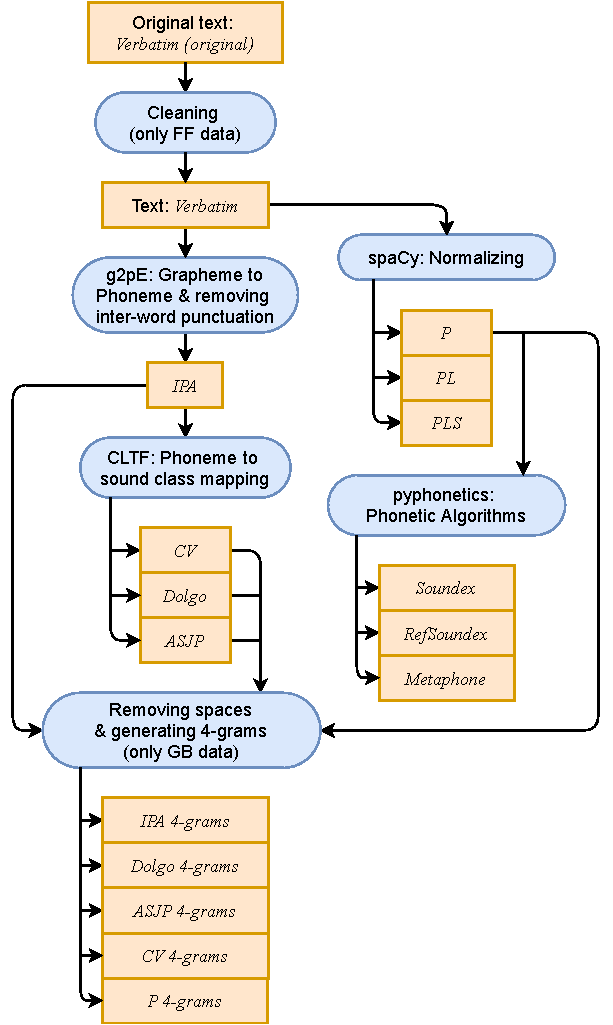
\includegraphics[width=0.7\textwidth]{figures/transcription}
  \caption{Transcription setup, orange = data, blue = process}
  \label{fig:transcription}
\end{figure}


% Statistical analysis
% Vocab reduction on some corpus
% Vocab size counting: Space Tokenize, count tokens that are not punctuation and are not numbers, upper- / lower-case is dismissed. This leaves soundex tokens in. Texts of a pair are concatenated
\section{Transcription Characteristics}
To better understand the characteristics of the phonetic transcription systems used, we conduct some preliminary investigations.
We calculate the vocabulary size scaling factor ($VSSF$) for each transcription system by determining the ratio of the number of distinct lexical types before and after transcribing.
A $VSSF$ of 1.5, for example, indicates that the transcription system examined increases the vocabulary size by 50\%.
This way, we can assess the granularity of the different transcription systems.
A vocabulary reduction of 50\%, for example, indicates that on average two words are binned into one transcription.
In practice, there might be many transcriptions which were transcribed from unique words and some transcriptions which group many words.
We calculate the absolute vocabulary size and the $VSSF$ per transcription system per dataset.
Table \ref{tab:system_characteristics} shows the results.\\
First, let us take a look at findings for the Gutenberg dataset, which are visualized in \ref{fig:vssf_transcriptions_gb}.
The $Verbatim$ text contains 50277 types.
Both $IPA$ and $ASJP$ increase the vocabulary size by a significant amount, 20.68\% and 11.21\% respectively.
This is to be expected as the alphabet of both systems is larger than the alphabet of verbatim text.
The text with removed punctuation ($P$) retains the same amount of types as punctuation symbols are not counted towards them.
By further lemmatizing the texts ($PL$), more tokens are binned and the resulting vocabulary is reduced by 18.6\%.
Eliminating stop words ($PLS$) removes 220 more types.
The $Dolgo$ system has an even smaller amount of types, but still retains more type granularity than the more simple phonetic algorithms.
$RefSoundex$ and $Metaphone$ reduce the vocabulary size by 41.44\% and 47.29\% respectively.
Because of its length restriction to four characters, $Soundex$ can at most produce 8,918 unique types (A000 to Z666) with only 4250 of them appearing in the data.
Lastly, $CV$ reduces the number of types the most and retains only 1954 types.
A reduction to 3.89\% of the original vocabulary size implies that on average ca.\ 26 words are binned to one transcription.\\

\begin{figure}
  \centering
  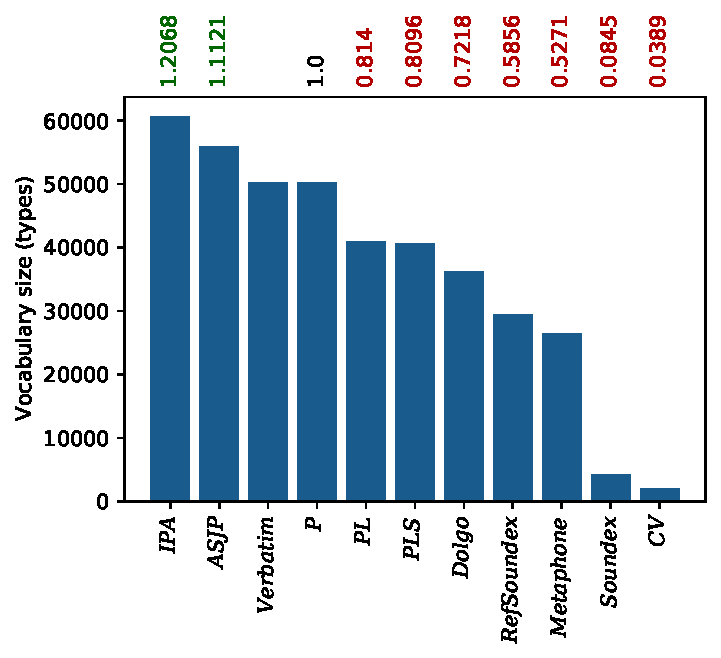
\includegraphics[width=0.7\textwidth]{figures/vocab_sizes_2021-07-28_14-42-08_gb_pt}
  \caption{Vocabulary sizes for transcriptions on Gutenberg dataset with $VSSFs$ above}
  \label{fig:vssf_transcriptions_gb}
\end{figure}
\begin{figure}
  \centering
  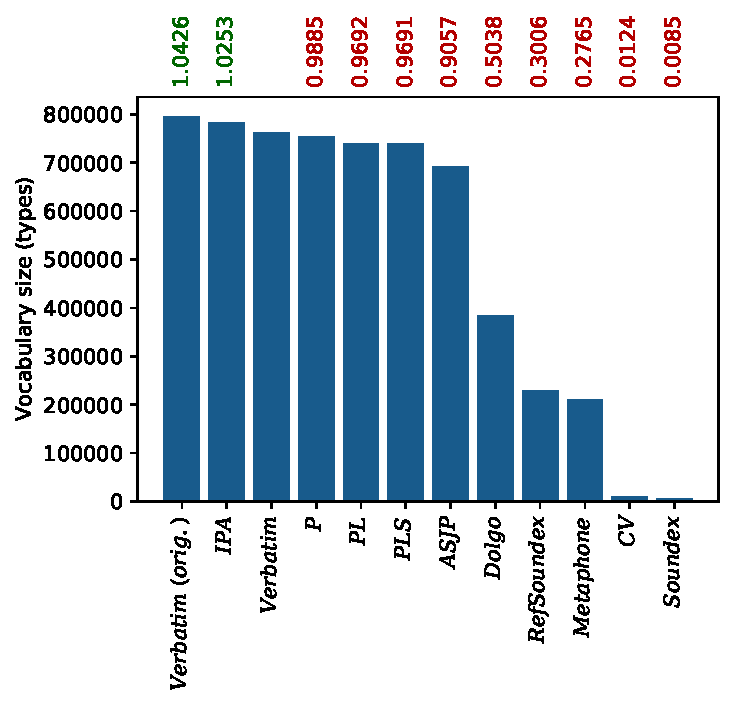
\includegraphics[width=0.7\textwidth]{figures/vocab_sizes_2021-07-27_16-57-38_ff_pt}
  \caption{Vocabulary sizes for transcriptions on Fan-fiction dataset with $VSSFs$ above}
  \label{fig:vssf_transcriptions_ff}
\end{figure}

Figure \ref{fig:vssf_transcriptions_ff} shows the results for the same analysis using the Fan-fiction dataset.
Both plots are predominantly similar but exhibit a few interesting differences.
Note that the the Fan-fiction dataset is substantially larger than the Gutenberg dataset.\\
The vocabulary size of the uncleaned (original) verbatim text is larger than that of the cleaned one.
This was expected as we removed certain words.




mainly similar
- remind: Looking at datasets of vastly different size -> Effects could and do stem from this
points
- verbatimoriginal is bigger: ok bc tokens / words were removed
- difference between verbatim and p: Probably bc of more noisy intra-word punctuation that is removed.
- lower! difference between p and pl/pls: Maybe lemmatizing isn't as effective on noisy data.
- Soundex lower than CV: Soundex is bound to 4, CV isn't

The most notable difference is that when transcribing the Gutenberg dataset $ASJP$ leads to an increase in vocabulary size whereas using the Fan-fiction dataset $ASJP$ surprisingly results in a significant reduction of the vocabulary.
It turns out that the cause for this phenomenon can be passed on to its preceding transcription, $IPA$.
The vocabulary reduction by mapping $IPA$ to $ASJP$ is 7.85\% for the Gutenberg dataset and 11.67\% for the Fan-fiction dataset.

dgb: 40.19\%
dff: 50.87\%

Adding random numbers cause it's late:
If we raise FF IPA increase to 20.68\%, where would ASJP land? above verbatim?
-> 0.8833 * 1.2068 = 1.06596644
 1.06596644 + (0.1167 - 0.0785) = 1.10416644 (vs. 1.1121)
-> Missing 4 percent coincide with increased ASJP decrease above.
Does this also work for Dolgo?
-> 0.4913 * 1.2068 = 0.59290084
->0.59290084 + (0.5087-0.4019) = 0.69970084 (vs. 0.7218)
meh, kinda


- ASJP is lower
- remind: verbatim -> IPA -> ASJP
- Only IPA ratio is different (calculate values)
- And in fact, it turns out that this is the case.


Outline:
Show Heap's law: GB (shuffled), GB sorted, FF sorted, FF shuffled
look at presentation: explain change of curvature
-> Show table of authors
present open problem: line non-divergence
Maybe mention in the beginning: "To get an idea of the transcription systems BUT ALSO OF THE DATASETS"

% Fan-fiction
% Most changes are ok, things are the same
% 1. ASJP moved down:
%   Difference in VSSF between IPA->Dolgo and IPA->ASJP are similar for both datasets.
%   -> Maybe Verbatim->IPA is the problem.
% 2. Lemmatization doesn't have a big impact anymore. Unclear why.
% 3. Soundex and CV switched places: prob. bc Soundex is capped, CV isn't


% {"ff": {"same_authors": 6397, "diff_authors": 47813, "same_diff_intersection": 1555, "same_text_per_author": 8.702204158199155, "diff_text_per_author": 1.035994394829858}, "gb": {"same_authors": 54, "diff_authors": 56, "same_diff_intersection": 53, "same_text_per_author": 4.814814814814815, "diff_text_per_author": 4.714285714285714}}

\begin{table}
\caption{Characteristics of the datasets used. TPA = texts per author.}
\label{tab:dataset_characteristics}
\centering\small
\begin{tabular}{@{}l@{\hspace{1\tabcolsep}}lll@{}} % Use @{\hspace{2\tabcolsep}} to double the spacing
\toprule
\bf  & \bf Gutenberg & \bf Fan-Fiction \\
\midrule
same-author authors & 54 & 6397 \\
different-author authors & 56 & 47813 \\
intersection & 53 & 1555 \\
same-author TPA & 4.8148 & 8.7022 \\
diff-author TPA & 4.7143 & 1.036 \\
\bottomrule
\end{tabular}
\end{table}




% Other statistics: text length (in characters)
% Other todo:
% Add function to count character length of text
% Maybe rename vocab_sizes.py to characteristics.py
% Change "properties" in text to "characteristics"

\newcommand{\specialcell}[2][c]{%
  \begin{tabular}[#1]{@{}c@{}}#2\end{tabular}}

\begin{table}
\caption{Characteristics of the transcription systems used. "Verbatim" represents original English text. Punctuation and whitespace not included in alphabet size. Alphabet sizes are theoretically derived.}
\label{tab:system_characteristics}
\centering\small
\begin{tabular}{@{}l@{\hspace{1\tabcolsep}}rlrlr@{}} % Use @{\hspace{2\tabcolsep}} to double the spacing
\toprule
\bf System & \bf \specialcell{GB\\absolute} & \bf \specialcell{GB\\VSSF} & \bf \specialcell{FF\\absolute} & \bf \specialcell{FF\\VSSF} & \bf Alphabet size \\
\midrule
$Verbatim$ $(orig.)$ & -- & -- & 795621 & 1.0426 & 26(?) \\
$IPA$ & 60673 & 1.2068 & 782424 & 1.0253 & >100(?) \\
$ASJP$ & 55913 & 1.1121 & 691146 & 0.9057 & 41(?) \\
$Verbatim$ & 50277 & 1.0 & 763097 & 1.0 & 26(?) \\
$P$ & 50277 & 1.0 & 754293 & 0.9885 & 26(?) \\
$PL$ & 40924 & 0.814 & 739629 & 0.9692 & 26(?) \\
$PLS$ & 40704 & 0.8096 & 739530 & 0.9691 & 26(?) \\
$Dolgo$ & 36288 & 0.7218 & 384440 & 0.5038 & 11 \\
$RefSoundex$ & 29441 & 0.5856 & 229360 & 0.3006 & 36 \\
$Metaphone$ & 26501 & 0.5271 & 210973 & 0.2765 & 21 \\
$Soundex$ & 4250 & 0.0845 & 6471 & 0.0085 & 32 \\
$CV$ & 1954 & 0.0389 & 9436 & 0.0124 & 2 \\
$IPA$ $4$-$grams$ & 176092 & 3.5024 & -- & -- & 2 \\
$P$ $4$-$grams$ & 103983 & 2.0682 & -- & -- & 2 \\
$ASJP$ $4$-$grams$ & 78246 & 1.5563 & -- & -- & 2 \\
$Dolgo$ $4$-$grams$ & 4061 & 0.0808 & -- & -- & 2 \\
$CV$ $4$-$grams$ & 16 & 0.0003 & -- & -- & 2 \\
\bottomrule
\end{tabular}
\end{table}






% Re Heaps Law FF:
% Why is there a sudden change of curvature in Verbatim text?
% -> Dataset is sorted: First same-author pairs, then different-author pairs
% BUUUUT: Even when pairs are split into single texts, the change in curvature still exists! (-> Maybe run again on remote, results now use naive split(' ') method on verbatim text)
% This may(!) be a good marker for assessing a bias in AV datasets: Sort dataset as above, determine heaps law coefficients.
% Check on GB dataset: Sort and plot Heaps Law -> No change of curvature!

% Question standing: Why is the individual vocab size still the same? Shouldn't it be higher?
% It doesn't need to be, but if the vocab sizes stay the same a change of curvature means that the vocabulary changes in itself.
% Might have to do with reusing authors or something.
% Check further: It seems that for FF in different-author part there are far more authors than for same-author part. Check if this is the same with GB.

% Why is the distance between Verbatim and IPA not getting larger in one part of the plot?